\section{Section header}

Given the length of each chapter, it is required to use headers and sub headers (possibly sub-sub headers).  These can be numbered or one can just rely on different formats.  The section headers in this document are labeled “heading 2” (“heading 1” was used for chapter titles).  The heading styles formats should be consistent throughout the document as it helps significantly in creating the automatic table of contents.

\subsection{Sub Heading}

The subheadings here have a different format (“heading 3”) than the section headers.

\subsubsection{Sub-Sub Heading}

You can even get to another level of headers, defined here as “heading 4.”  The table of contents, however, is currently set up to just include three levels of headers.

\subsection{Equations}

Equations can be created in MS WORD equation editor or they can be created with other software.  Equations should be numbered.  They can be numbered within each chapter (e.g., 2.1, 2.2) or they can be numbered sequentially throughout the entire thesis.  Equations should be indented or centered with the equation number to the right.  The example below and associated “thesis-eqn” style can be used for all your equations.

\todo{Include example of an equation here.}

This equation was written with the equation editor. Found through “insert, object, equation editor 3.0. The equation editor can also be found through “tools, customize, commands”, and in categories, look for insert and in the commands section, look for equation editor, drag and drop the icon onto the toolbar. This editor is fine for relatively simple equations, other options are available for more complex equations.

\subsection{Tables}

Tables should have meaningful information with descriptive headers.  You can use the “thesis-table caption” style to define your captions and refer to the table in the text with a “cross reference” (Table 1).  MS Word re-numbers table captions automatically when new tables inserted.  But you need to right click on any cross references and “update field” if there are changes.

\begin{table}[h!]
  \centering
  \begin{tabularx}{0.8\textwidth} {
    | >{\centering\arraybackslash}X 
    | >{\centering\arraybackslash}X 
    | >{\centering\arraybackslash}X |
  }
    \hline
      Step \# & Instruction \\ 
    \hline
      Create table caption & Insert, reference, caption, table \\ 
    \hline
      Format the caption & Format, style, “thesis-table-caption” \\ 
    \hline
      Create table & Table, insert… \\
    \hline
      Format the table & The formatting of the table can vary, including use of single space as appropriate. Most journals require that tables are formatted using table style “Table Simple 1” format. \\
    \hline
      Reference the table from text & With the cursor at the location you want to cite the table: insert, reference, cross reference, table, label and number only. \\
    \hline
  \end{tabularx}
  \caption{Table 1: Steps in creating a table}
  \label{table:1}
\end{table}

\subsection{Figures}

Figures and illustrations are a necessary means of communicating technical information.  Often times, figures included in the background/lit review section are copied from existing copyrighted information.  In all cases, this is technically inappropriate without also receiving permission from the copyright owner.  Citing the source of the figure is not sufficient. This rule is enforced for PhD dissertations because they are submitted to ProQuest for electronic access by others.  The enforcement of this rule for MS theses is dependent on the specific committee members.

Resolution of figures is often a problem in theses.  Resolution should be >300 dpi, preferably 600dpi (\ref{fig:figure1}).  You should note that saving images as jpeg files is a sure way to lower the resolution to an unacceptable extent.  From experience, a good way is to copy your graphic (for example from PowerPoint or excel) and when pasting it into word, use the “paste special” “as an “enhanced metafile” (\ref{fig:figure2}).  This also substantially reduces the resulting file size in comparison with pasting graphs in as excel graphics.

\begin{figure}
  \centering
  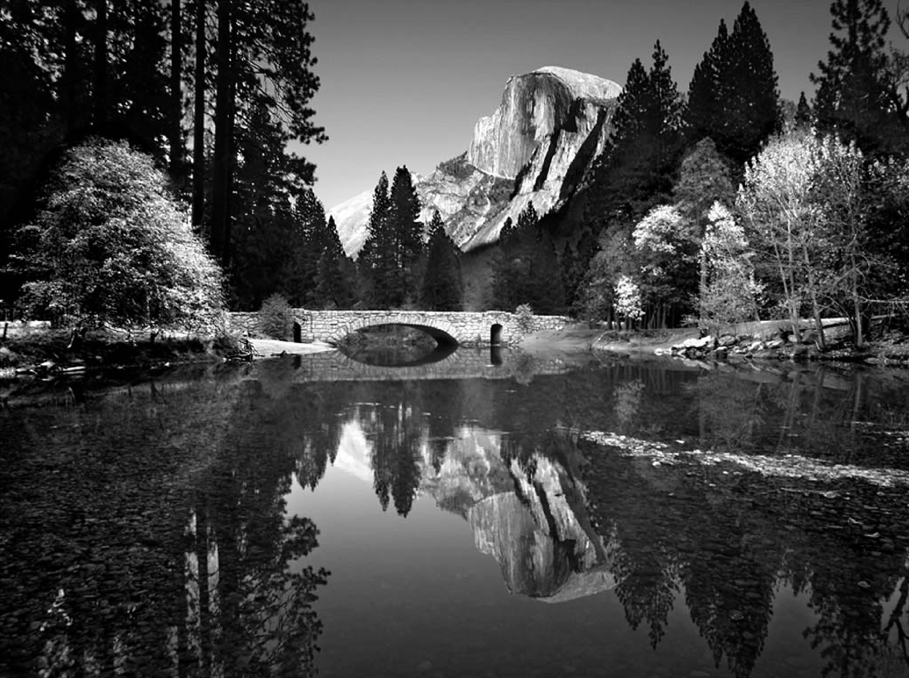
\includegraphics[width=0.8\textwidth]{Figure1}
  \caption{Figure 1: Example photo with high resolution.  Caption created with ``insert, reference, caption, figure'' and the style changed to ``thesis-figure caption.''}
  \label{fig:figure1}
\end{figure}

\begin{figure}
  \centering
  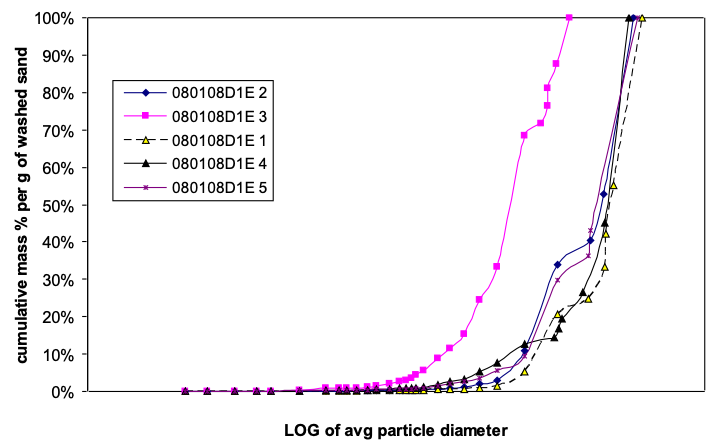
\includegraphics[width=0.8\textwidth]{Figure2}
  \caption{``Figure 2: Example of high resolution graphic inserted with “paste special, as enhanced metafile''}
  \label{fig:figure2}
\end{figure}
